\PassOptionsToPackage{fontset=macnew}{CTEX}
\documentclass[10.5pt,compsoc,UTF8]{CjC}
\usepackage{CTEX}
\usepackage{graphicx}
\usepackage{url}
\usepackage{multirow}
\usepackage{multicol}
\usepackage[noadjust]{cite}
\usepackage{amsmath,amssymb}
\usepackage{booktabs}
\usepackage{float}
\usepackage{fancyhdr}
\usepackage{caption}
\usepackage{xcolor,stfloats}
\usepackage{gbt7714}
\usepackage{array}
\graphicspath{{./}}
\setcounter{page}{1}
\headevenname{\zihao{-5}计\quad 算\quad 机\quad 学\quad 报}
\headoddname{课程设计报告\hfill 台风分类与路径预测}
\renewcommand{\thefootnote}{\fnsymbol{footnote}}
\renewcommand{\figurename}{图}
\newcommand{\upcite}[1]{\textsuperscript{\cite{#1}}}
\renewcommand{\bibsection}{}
\setlength\parindent{2em}
\pagestyle{CjCheadings}
\setmainfont{Times New Roman}
\begin{document}
\hyphenpenalty=50000
\thispagestyle{empty}
\begin{table*}[!t]\vspace{-13mm}\onecolumn\noindent\begin{tabular}{p{168mm}}
\zihao{5-}课程设计报告\hfill 机器学习\hfill 2026 年\\[-1mm]\hline\hline\end{tabular}\end{table*}
{\centering\vspace{8mm}{\zihao{2}\heiti 基于机器学习的台风分类、路径预测与降水衰减分析}\vskip 4mm
{\zihao{4}\fangsong 徐诗霖(202622080929)\quad 蔡奕锴(202622080928)\quad 李炜焜(202622080705)}\footnote{\zihao{6}\songti 作者：徐诗霖(202622080929)、蔡奕锴(202622080928)、李炜焜(202622080705)，电子科技大学，机器学习课程设计。}\vspace{1mm}
\zihao{6}{$^{1)}$(电子科技大学，成都 611731)}\par}
\vskip 4mm
\zihao{5-}{\setlength{\baselineskip}{16pt}\selectfont{\noindent{\heiti 摘要}\quad 台风分类、路径预测和登陆后影响评估是机器学习服务于灾害预警的典型任务。本文以历史台风样本和2024年第13号台风贝碧嘉观测数据为对象，完成一份开题研究内容的总结性报告。首先对经纬度、气压、风速、移动速度和等级等变量进行缺失值处理、异常检查与标准化，结合相关性分析和主成分分析提取主要特征，并用K均值聚类识别台风类别。其次，构建支持向量回归与CNN-LSTM相结合的路径预测流程，以动态时间规整（DTW）和均方根误差（RMSE）评价预测轨迹。最后，以风速、台风中心距离和降水量为变量，比较幂律、指数衰减及综合模型，分析登陆后降水的时空变化。结果表明：风速与等级高度正相关（相关系数0.9961），气压与风速强负相关（-0.9433），肘部法确定聚类数为3；路径预测示例的RMSE为0.23167、DTW距离为94.2486；综合模型能较好刻画贝碧嘉登陆后降水快速下降并趋于平稳的过程。研究为后续扩充数据、改进时空特征建模和开展实时预警提供基础。\par}}
\vspace{3mm}\zihao{5-}{\noindent{\heiti 关键词}\quad 台风分类；路径预测；支持向量回归；卷积神经网络；长短期记忆网络；动态时间规整；降水衰减}\par
\zihao{5-}{\noindent{\heiti 中图法分类号}\quad TP181\par}
\vskip 3mm
\begin{center}\zihao{3}\heiti Machine-learning-based Typhoon Classification, Track Prediction and Precipitation Decay Analysis\\[3mm]
\zihao{5} SHI-LIN XU, YI-KAI CAI, WEI-KUN LI\\[1mm]\zihao{6}{$^{1)}$(University of Electronic Science and Technology of China, Chengdu 611731)}\end{center}
\zihao{5}{\noindent\textbf{Abstract}\quad Typhoon early warning requires a joint understanding of intensity, track and post-landfall hazards. Using historical typhoon records and observations of Typhoon Bebinca in 2024, this study summarizes a machine-learning research design. Missing values and outliers are processed before correlation analysis, principal component analysis and K-means clustering. A support vector regression and CNN-LSTM pipeline is then used for track prediction, with dynamic time warping (DTW) and root mean square error (RMSE) as evaluation metrics. For post-landfall impacts, power-law, exponential-decay and combined models are compared to describe the relationships among wind speed, distance to the center and precipitation. Wind speed is highly correlated with typhoon grade (0.9961) and negatively correlated with pressure (-0.9433). The elbow method selects three clusters. In the representative track experiment, RMSE is 0.23167 and DTW distance is 94.2486. The combined model captures the rapid decrease and later stabilization of precipitation after landfall. The study provides a compact and reproducible basis for future real-time warning systems.\par}
\vspace{3mm}\zihao{5}{\noindent\textbf{Keywords}\quad typhoon classification; track prediction; support vector regression; convolutional neural network; long short-term memory; dynamic time warping; precipitation decay\par}
\vskip 2mm
\begin{multicols}{2}
\section{引言}
台风同时具有强非线性、长时间依赖和明显空间影响，其风速、气压和移动轨迹直接关系到防灾减灾决策。传统数值预报能够描述大尺度动力过程（如科里奥利力与风场、海温的耦合作用\upcite{wie2012development}），但对局地观测噪声、样本异质性和快速转向的适应仍有限。机器学习可从历史观测中学习变量之间的非线性关系\upcite{vapnik1998statistical,goodfellow2016deep}，并与物理启发的统计模型结合，形成轻量、可评估的预测流程。已有研究表明，深度学习和混合模型适合捕捉台风路径的时序特征\upcite{陈睿2018基于深度学习的台风预测关键技术研究,chen2019hybrid}，而DTW可在时间步不完全对应时评价两条轨迹的形状相似性\upcite{muller2007dynamic}。

本文将原有竞赛解答压缩为课程设计报告，围绕三个相互衔接的问题展开：\textbf{（1）}利用历史台风数据提取特征并进行分类；\textbf{（2）}以贝碧嘉为案例预测短期移动路径；\textbf{（3）}解释登陆后风速与降水量的衰减关系。报告重点说明数据流程、模型选择、评价指标和可复现结果，删去大段推导与代码附录。

\section{相关工作}
台风路径预测的机器学习方法可大致分为时序建模与多源融合两类。Gao 等（2018）用长短期记忆网络开展 6--24 小时路径预报，验证了历史序列时间依赖的预测价值；Giffard-Roisin 等\upcite{giffardroisin2020tropical}将历史位移与以台风中心对齐的风场、位势高度场融合，直接预测 24 小时位移；Liu 等（2022）提出 CNN-LSTM 双分支时空融合网络，实现多时效路径预测；R{\"u}ttgers 等用生成对抗网络结合卫星图像预测台风轨迹\upcite{ruttgers2019prediction}；Chen 等用 CNN-LSTM 进行台风生成与强度预测\upcite{chen2019hybrid}；He 等提出双注意力 ConvLSTM 用于短时风速预测\upcite{he2022dual}。在降水方面，Ueno\upcite{ueno2007observational}指出环境风切变会造成台风内核降水的空间不对称性。

综合来看，前人工作仍存在不足：\textbf{（1）}时序变化与环境因素的联合刻画不足，模型在转向与快速变速时存在偏差和滞后；\textbf{（2）}部分方法以移动速度而非未来位移为输出，预测目标与路径预测任务衔接不够清晰；\textbf{（3）}数据划分与评价指标不够严格，同一台风的相邻样本跨集合会造成信息泄漏；\textbf{（4）}登陆后降水模型多基于合成数据，缺乏真实观测依据。针对这些不足，本文采用“历史序列建模、直接预测位移、独立事件验证”的路线，并以真实观测数据检验降水衰减关系。

\section{数据与研究流程}
\subsection{数据描述}
数据采用国际热带气旋最佳路径档案（IBTrACS）\upcite{knapp2010ibtracs}中的历史台风记录（1945年至今），以及2024年7月、9月样本和贝碧嘉2024年9月13--19日的观测数据。核心变量为经度$\lambda$、纬度$\phi$、中心气压$P$、最大风速$V$、移动速度$S$、台风等级$G$、观测时间$t$和累积降水量$R$。数据按时间排序后，以相邻观测点补全移动方向和速度；对关键字段缺失的记录剔除，并采用标准化
\begin{equation}
z=(x-\mu)/\sigma
\end{equation}
消除量纲差异。异常值通过物理范围和箱线图联合检查，避免极端错误记录主导聚类和回归。

\subsection{符号说明}
本文主要符号见表\ref{tab:symbol}。
\begin{table}[H]\centering\small\caption{主要符号说明}\label{tab:symbol}
\begin{tabular}{cl}
\toprule
符号 & 含义\\
\midrule
$\lambda,\phi$ & 台风中心的经度与纬度\\
$P$ & 中心气压（hPa）\\
$V$ & 最大风速（m/s）\\
$S$ & 移动速度（m/s）\\
$G$ & 台风等级\\
$R$ & 累积降水量（mm）\\
$D$ & 观测点到台风中心距离（km）\\
$K$ & 聚类数\\
$J$ & 簇内平方误差（SSE）\\
\bottomrule
\end{tabular}
\end{table}

\subsection{总体流程}
研究流程为“数据清洗—探索分析—特征降维—分类—路径预测—登陆后影响拟合—误差分析”。分类结果用于观察夏、秋季台风差异；路径模型使用历史轨迹与气象特征；降水模型则聚焦贝碧嘉登陆后的短时间窗口。三部分共享标准化和交叉验证原则，但分别采用适合无监督、时序和回归问题的评价指标。

\section{台风特征分类}
\subsection{相关性与降维}
皮尔逊相关分析显示，风速与台风等级的相关系数为0.9961，气压与风速为-0.9433，气压与等级为-0.9422，说明风速和气压是强度判别的主要信息源；移动速度与多数强度变量相关性较弱，可能受引导气流和地理环境影响。图\ref{fig:heat}给出变量相关性概览。K-S检验显示多数变量不服从正态分布，故后续采用对分布假设不敏感的统计与机器学习方法。对标准化变量进行主成分分析（PCA）\upcite{abdi2010principal,jolliffe2002principal}，将高度相关的变量压缩为少数互不相关的主成分，降低聚类中的冗余。
\begin{figure}[H]\centering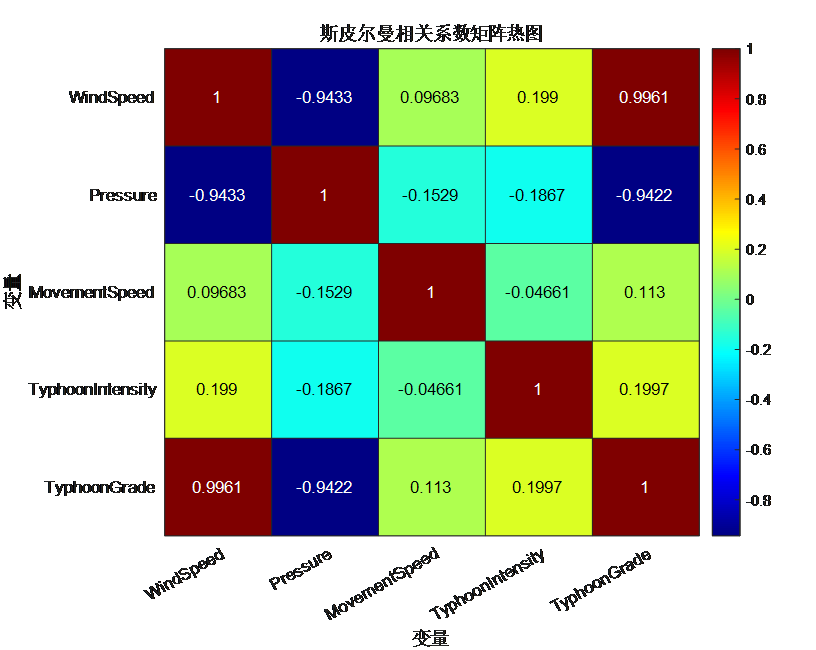
\includegraphics[width=\columnwidth]{热力图.png}\caption{主要变量相关性热力图}\label{fig:heat}\end{figure}

\subsection{K均值分类}
采用欧氏距离的K均值聚类\upcite{macqueen1967some}最小化簇内平方误差：
\begin{equation}J=\sum_{k=1}^{K}\sum_{x_i\in C_k}\lVert x_i-\mu_k\rVert^2.
\end{equation}
通过肘部法比较不同$K$的SSE，曲线在$K=3$后下降趋缓（图\ref{fig:elbow}），因此选择三类，并以轮廓系数\upcite{rousseeuw1987silhouettes}辅助验证聚类紧密度。聚类结果可解释为低强度、过渡型和高强度样本。图\ref{fig:cluster}给出经PCA投影后样本在二维主成分空间中的分布，三类形成可区分但边界有重叠的结构，说明单一强度指标不足以完全划分台风类别。
\begin{figure}[H]\centering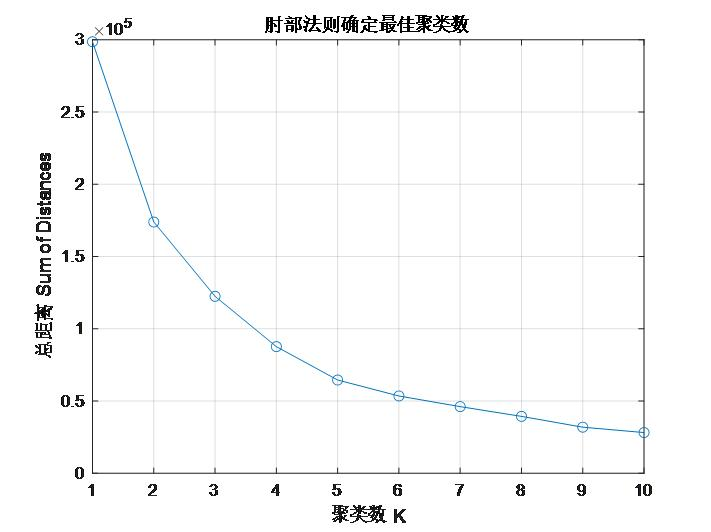
\includegraphics[width=\columnwidth]{肘部法.jpg}\caption{肘部法选择聚类数}\label{fig:elbow}\end{figure}
\begin{figure}[H]\centering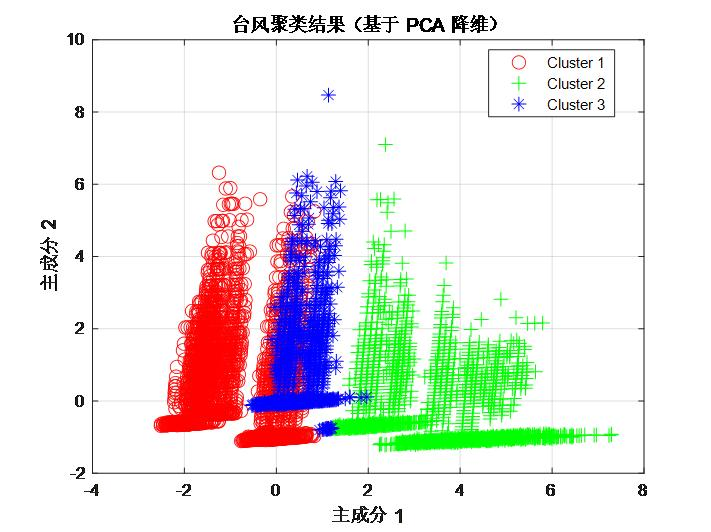
\includegraphics[width=\columnwidth]{台风聚类的结果.jpg}\caption{PCA投影下的台风聚类结果}\label{fig:cluster}\end{figure}

在无监督聚类揭示样本结构的基础上，进一步以决策树、支持向量机（SVM）\upcite{cortes1995support}和LSTM构建监督分类模型，比较不同算法对台风等级的判别能力，从而在无监督探索与有监督判别之间形成互补。表\ref{tab:season}给出夏、秋台风在关键特征上的对比。

夏季台风整体风速与等级偏高、多生成于低纬度并向西北方向移动，秋季台风强度略弱、路径更分散，但两季均表现出低气压与较强风速相联系的规律。这可解释为夏季高海温提供更多能量，而秋季季风扰动使路径更复杂。
\begin{table}[H]\centering\small\caption{夏、秋台风特征对比}\label{tab:season}
\begin{tabular}{lcc}
\toprule
特征 & 夏台风 & 秋台风\\
\midrule
风速与等级 & 偏高 & 偏低\\
气压 & 受低压条件控制 & 相似\\
生成位置 & 多位于低纬度 & 多位于较高纬度\\
强度 & 较强 & 较弱\\
路径特点 & 向西北移动 & 更分散\\
\bottomrule
\end{tabular}
\end{table}

生成台风路径如图\ref{fig:paths}所示，夏季台风路径多向西北方向移动，秋季路径更分散，与表\ref{tab:season}的统计特征一致。
\begin{figure}[H]\centering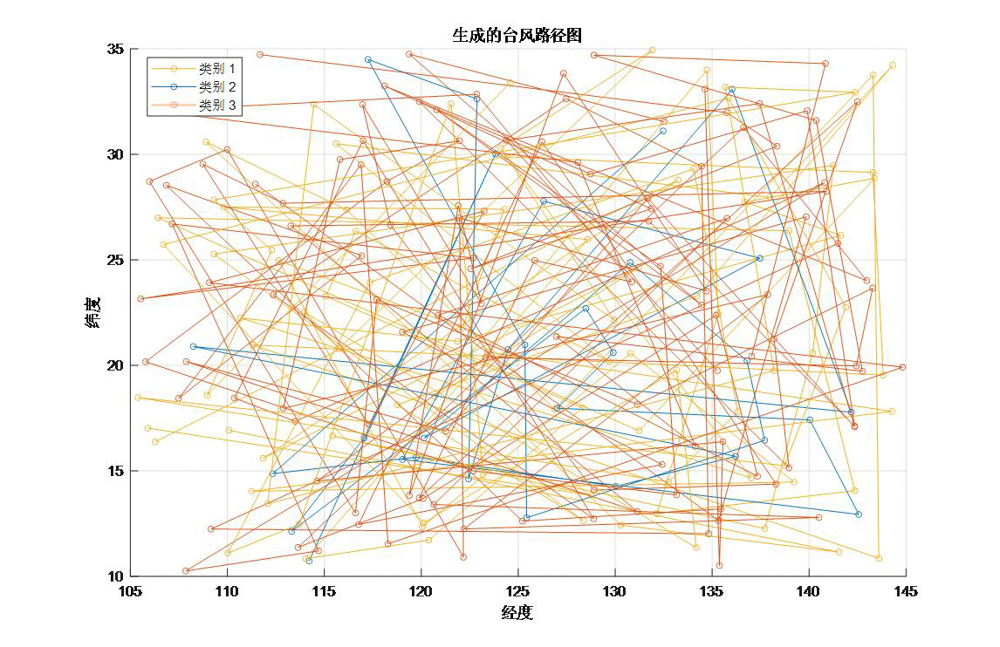
\includegraphics[width=\columnwidth]{生成台风路径图.jpg}\caption{生成台风路径的空间分布}\label{fig:paths}\end{figure}

\section{贝碧嘉路径预测}
\subsection{模型设计}
将经纬度序列和气象变量构造成滑动时间窗，构建“SVR基线—CNN-LSTM—通道注意力”的递进式预测流程。SVR通过核函数把低维非线性关系映射到高维空间，其预测函数为
\begin{equation}f(x)=\sum_{i=1}^{n}(\alpha_i-\alpha_i^{*})K(x_i,x)+b,
\end{equation}
其中$K(\cdot,\cdot)$为径向基核函数，$\alpha_i,\alpha_i^{*}$为拉格朗日乘子，$b$为偏置项\upcite{cortes1995support,drucker1997support,dhiman2019hybrid}。CNN在时间窗上提取局部变化模式，LSTM通过遗忘门、输入门和输出门刻画长期依赖，缓解普通循环网络的长序列梯度问题\upcite{hochreiter1997long}；两者融合构成时空表达，再以通道注意力机制对关键气象特征加权\upcite{lecun2015deep}（图\ref{fig:arch}）。
\begin{figure}[H]\centering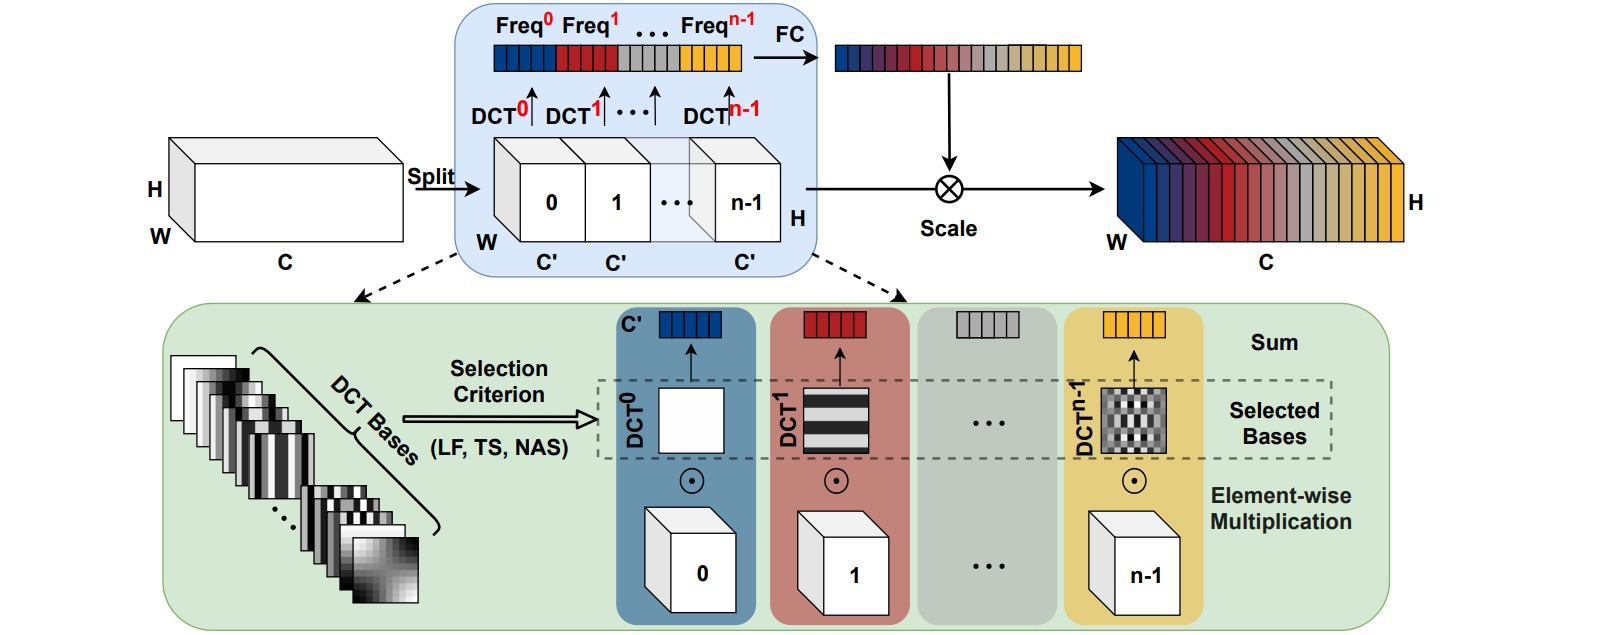
\includegraphics[width=\columnwidth]{神经网络通道图.jpg}\caption{CNN-LSTM与通道注意力结构示意}\label{fig:arch}\end{figure}

网络采用Adam优化器训练\upcite{kingma2014adam}，训练集、验证集和测试集按时间划分，避免未来信息泄漏。路径点误差采用RMSE：
\begin{equation}\mathrm{RMSE}=\sqrt{\frac{1}{n}\sum_{i=1}^{n}(\hat y_i-y_i)^2}.
\end{equation}
对预测和实际轨迹分别按时间排列，DTW通过允许局部拉伸或压缩求最小累积距离\upcite{muller2007dynamic,sakoe1978dynamic}，补偿观测间隔不一致的影响。

\subsection{结果与分析}
图\ref{fig:path}展示代表性预测轨迹。实验得到RMSE=0.23167、DTW距离=94.2486，其中RMSE对较大误差更敏感、适合突出预测偏差\upcite{willmott2005advantages}。整体趋势与实际路径一致，误差主要出现在转向和移动速度突变区间。训练、验证和测试误差分布总体集中，说明模型未出现明显的过拟合，但测试集尾部仍有较大误差；误差在经度130°--140°的转向区间和高移动速度样本上偏高，说明模型对剧烈转向与快速变速的时间依赖刻画仍不充分。该结果支持“SVR提供稳健基线、CNN-LSTM补充时序表达、DTW评价轨迹形状”的组合方案。
\begin{figure}[H]\centering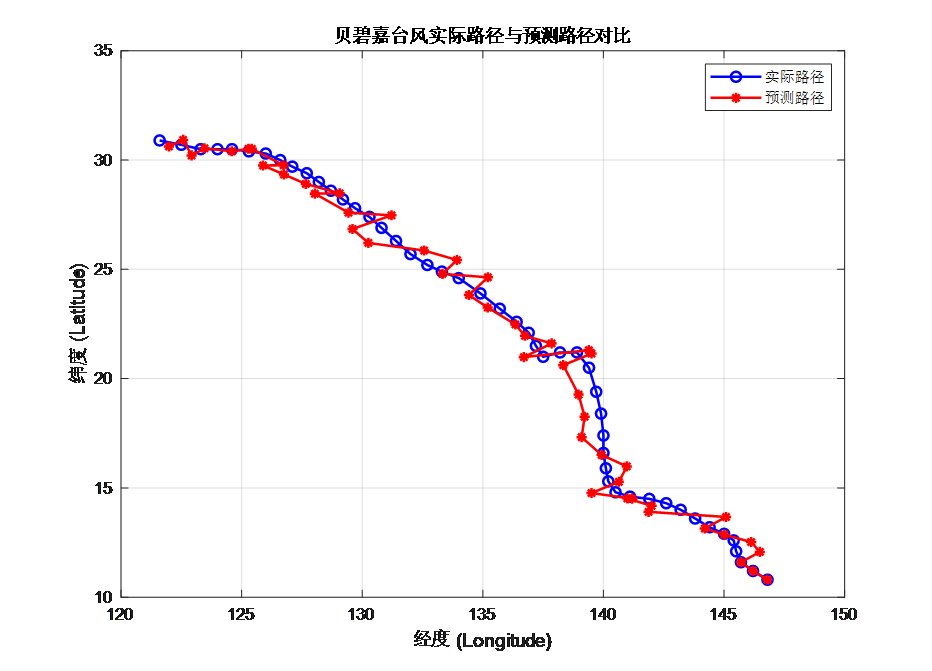
\includegraphics[width=\columnwidth]{路径对比图.png}\caption{贝碧嘉预测路径与实际路径对比}\label{fig:path}\end{figure}

图\ref{fig:err}给出训练集、验证集和测试集的预测误差分布，三者分布总体集中、无系统性偏移，说明模型未过拟合；测试集误差略宽，尾部存在少量较大误差样本。图\ref{fig:speed}比较实际移动速度与预测移动速度，散点呈明显正相关，时序上两条曲线趋势一致，但在高速度与剧烈加减速区间偏差较大，这与路径预测在转向区间的误差来源一致。
\begin{figure}[H]\centering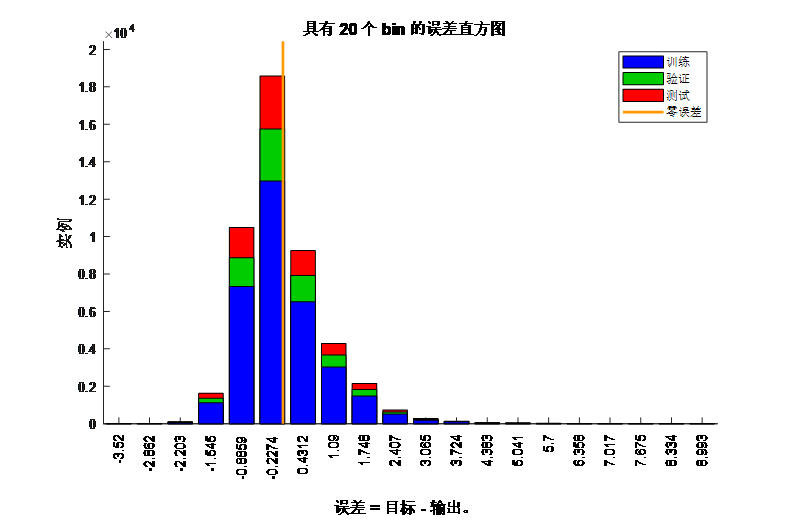
\includegraphics[width=\columnwidth]{误差图.png}\caption{训练、验证与测试集的误差分布}\label{fig:err}\end{figure}
\begin{figure}[H]\centering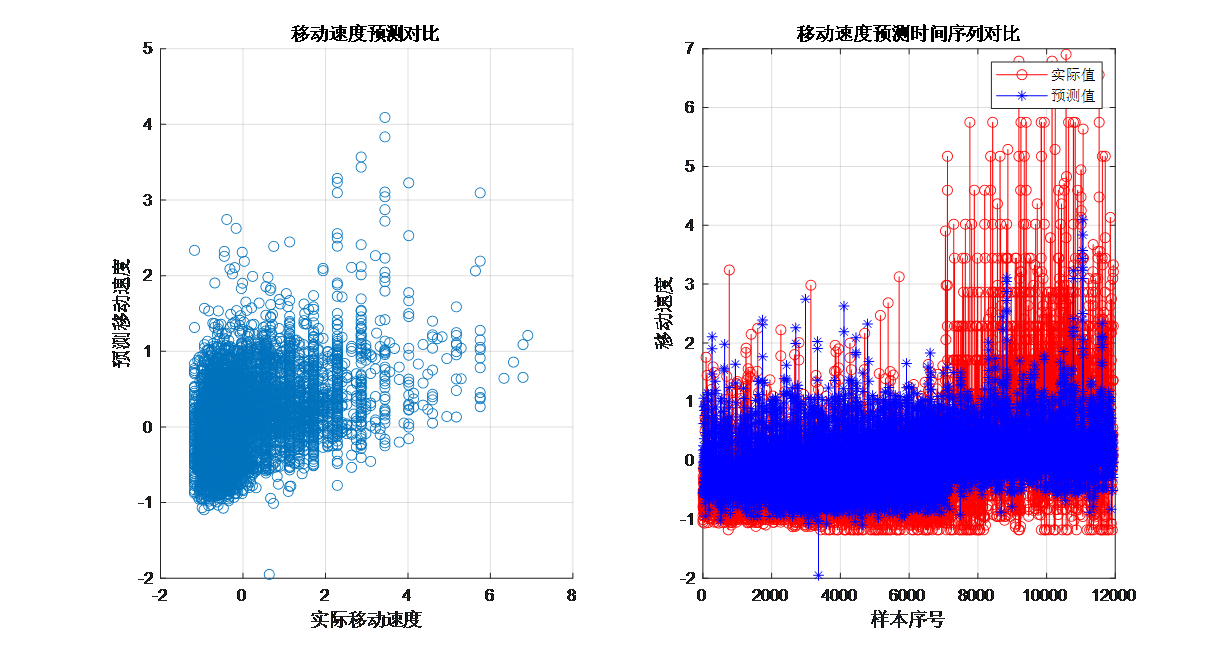
\includegraphics[width=\columnwidth]{移动速度和时间序列对比图.png}\caption{移动速度预测与实际对比}\label{fig:speed}\end{figure}

\section{登陆后风速与降水衰减}
\subsection{关系模型}
台风登陆后因海洋能量供给中断，风速与降水量总体下降，其衰减过程可用经验模型刻画\upcite{kaplan1995simple}。二者存在动力学与热力学两重联系：高风速增强对流与水汽凝结，同时增大海面蒸发、补充水汽。定量刻画时，对风速与降水量采用幂律关系
\begin{equation}R=aV^b+\varepsilon,
\end{equation}
对中心距离采用指数衰减
\begin{equation}R(D)=R_0\exp(-D/L)+\varepsilon,
\end{equation}
其中$D$为观测点到台风中心的距离，$L$为衰减尺度，$\varepsilon$表示观测噪声。除上述单变量模型外，进一步引入高斯模型$R=R_0\exp[-(D-\mu)^2/(2\sigma^2)]$和多项式模型，并用最小二乘、随机森林\upcite{breiman2001random,freund1997decision,friedman2001greedy}与高斯过程回归\upcite{williams2006gaussian,schulz2018tutorial}等多变量方法联合气压、温度和时间特征，参数估计与拟合优度评价遵循曲线拟合一般原则\upcite{motulsky2004fitting}。综合模型以残差、MSE和RMSE评价拟合质量。

\subsection{案例结果}
图\ref{fig:met}给出贝碧嘉登陆后风速、距离、温度和气压的时序变化：9月16--19日风速由约40 m/s降至约10 m/s，观测点到台风中心距离由约50 km增大到150 km，气压在950--1000 hPa间波动，反映出台风登陆后能量逐步耗散的过程。图\ref{fig:fit}表明风速增加时降水量总体增加，而距离中心增大时累积降水量下降；残差在高风速和快速转向阶段更分散。对2024年9月16--19日贝碧嘉数据的四种模型比较显示，单一条件、指数和高斯模型难以同时刻画初期快速下降与后期平稳，综合模型能更好保留该变化形态（图\ref{fig:rain}）。因此，降水风险评估宜将强度、距离和时间联合建模，而不应只依赖单变量衰减。
\begin{figure}[H]\centering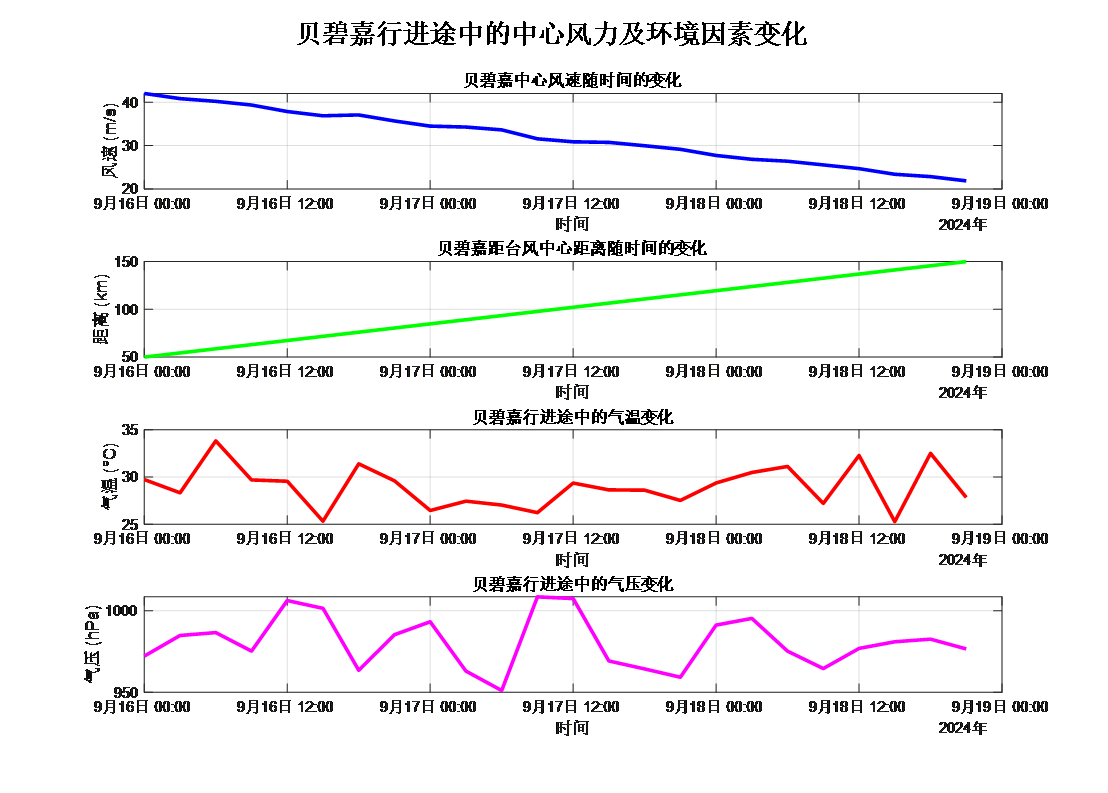
\includegraphics[width=\columnwidth]{台风贝碧嘉的气象变化分析.png}\caption{贝碧嘉登陆后气象变量时序变化}\label{fig:met}\end{figure}
\begin{figure}[H]\centering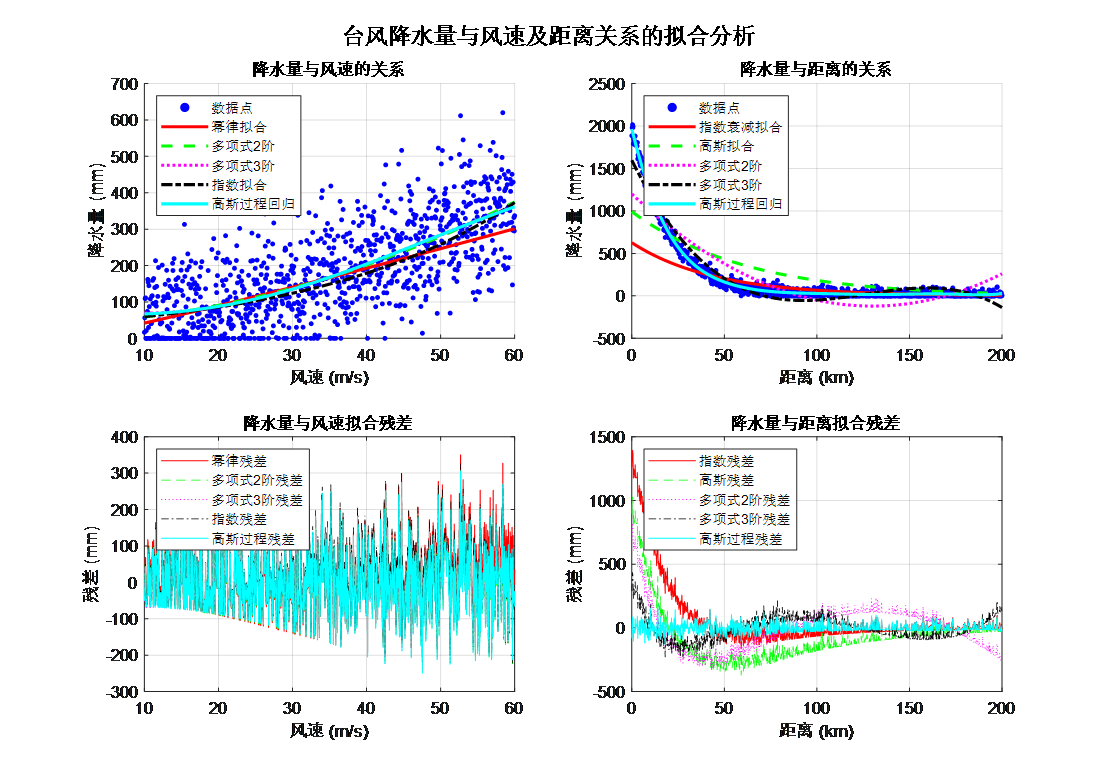
\includegraphics[width=\columnwidth]{台风降水量与风速及距离关系的拟合.png}\caption{风速、距离与降水量关系拟合}\label{fig:fit}\end{figure}
\begin{figure}[H]\centering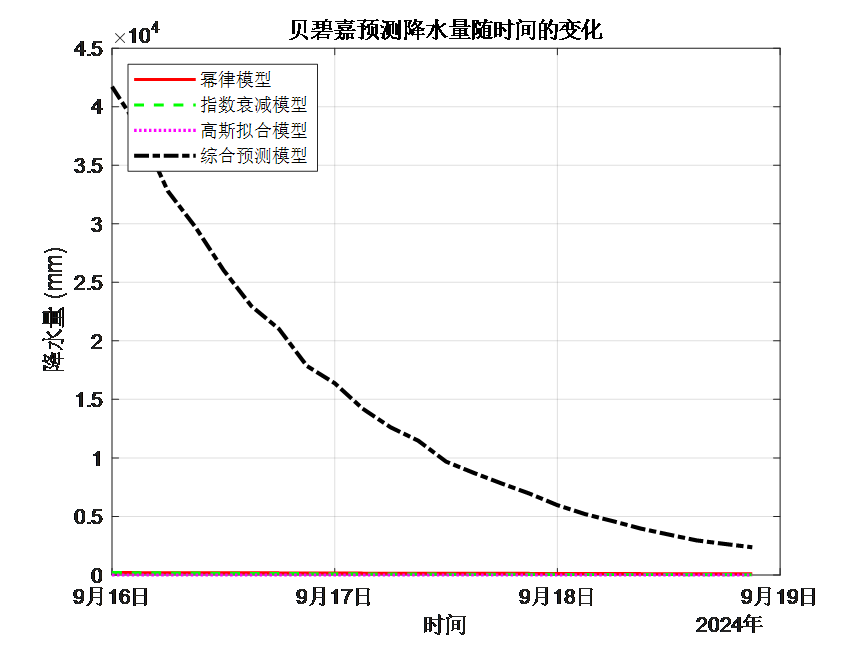
\includegraphics[width=\columnwidth]{贝碧嘉台风预测降水量变化.png}\caption{不同模型的贝碧嘉降水预测}\label{fig:rain}\end{figure}

图\ref{fig:resid}给出模型预测降水量与实际降水量的残差分析，残差在零线附近均匀分布、正负对称，无明显系统性偏差，说明综合模型整体无偏。
\begin{figure}[H]\centering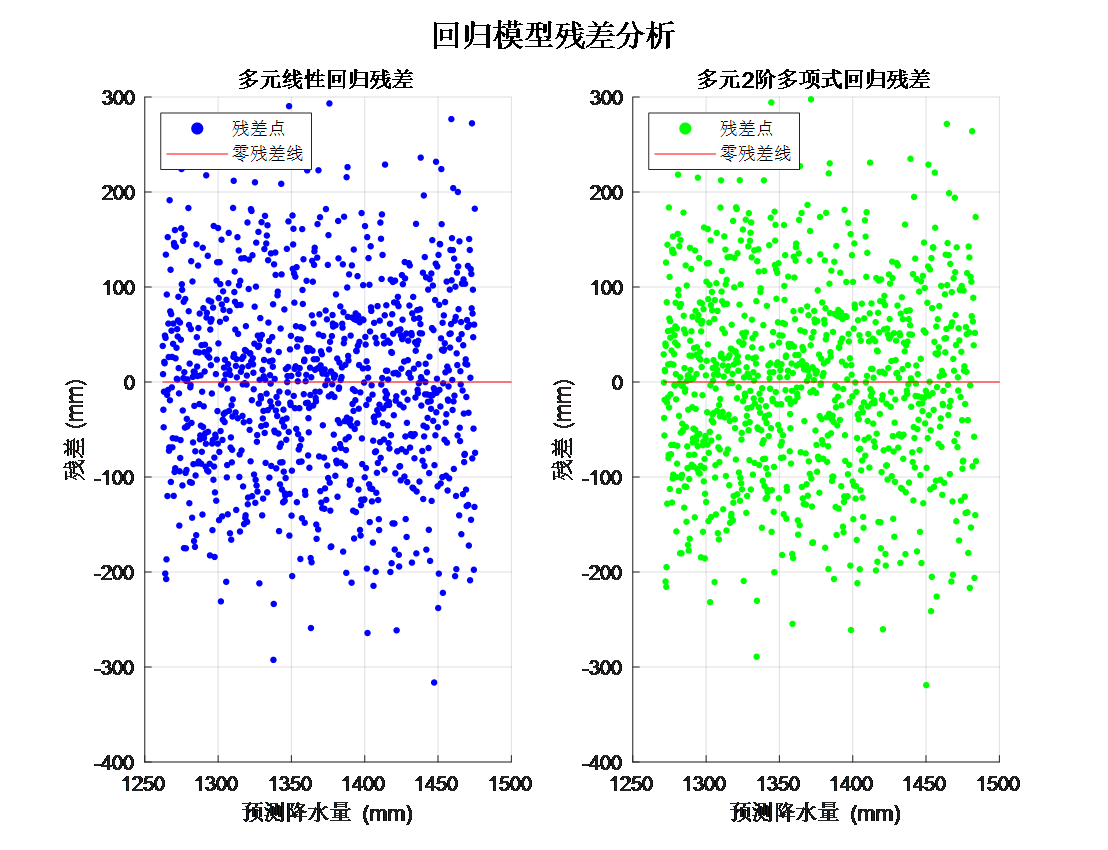
\includegraphics[width=\columnwidth]{模型预测降水量与实际降水量的比较.png}\caption{模型预测降水量与实际降水量比较}\label{fig:resid}\end{figure}

\section{讨论与结论}
本文将三个研究任务统一到一个可复现的机器学习流程中。分类阶段给出了可解释的变量关系和三类聚类结构；路径阶段用SVR与CNN-LSTM结合，获得RMSE和DTW两种互补评价；降水阶段通过幂律、指数和综合模型刻画登陆后的影响变化。

从方法上看，本方案具有三点优势：一是多变量融合，综合模型整合风速、气压、温度与距离等输入，通过不同模型的优势互补提升预测精度；二是评价指标互补，RMSE度量逐点误差、DTW度量轨迹形状，二者结合能更全面地刻画预测质量；三是可解释性较强，相关分析与聚类给出了清晰的变量关系和类别结构，便于后续风险分级。主要局限包括：历史样本与观测站点分布不均，部分变量存在强共线性；案例评估集中于单个台风，结论的统计稳健性有限；尚未引入完整的海温、风场和地形栅格数据，且对台风剧烈转向与快速变速的时间依赖刻画仍不充分。

后续工作可从三方面推进：扩大独立测试台风数量以检验泛化能力；引入物理约束、注意力机制与不确定性估计，改善转向区间的预测；以滚动更新方式接入实时观测，支撑短临预警。总体而言，研究内容已形成“分类识别—路径预测—影响评估”的闭环，能够支撑机器学习课程设计对数据预处理、无监督学习、深度时序建模和回归评价的综合要求。

\vspace{2mm}\centerline{\zihao{5}\heiti 参 考 文 献}
\zihao{5-}\addtolength{\itemsep}{-1em}\bibliographystyle{gbt7714-numerical}\bibliography{ref.bib}
\end{multicols}
\end{document}
